\subsection{Diameter} \label{diameter}
In graph theory, \textit{shortest path}\cite{diameter} (SP)
between node $a$ and $b$ of a graph is the minimum number of
edges connecting them (i.e. the minimum number of ``steps'' to go
from node $a$ to $b$).\\
After computing SP for every couple of nodes in a graph, we can
define \textit{diameter}\cite{diameter} as the maximum of the
shortest paths.\\
As with clustering, we ran five simulations for every memory
size, obtaining a plot of diameter's mean with errors.
Final regression will point out possible correlations.
\begin{figure}[h]
  \centering
  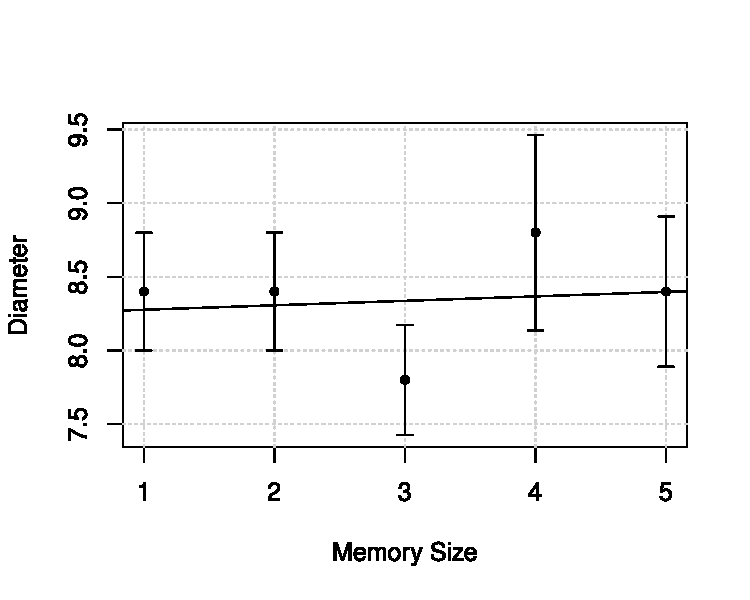
\includegraphics[trim={0cm 0cm 0cm 1cm},clip,width=.8\columnwidth]{img/diameter.pdf}
  \caption[Diameter's mean over memory size]
  {Diameter's mean over memory size plot with linear weighted fit:
    five simulations per point.}
  \label{fig:diameter}
\end{figure}
\begin{table}[h]
\label{tab:clusteringdiameter}
\centering
\begin{tabular}{r|cccc}
\toprule
& Slope & Intercept & $R^2$ & $\rho_{xy}$ \\
\midrule
\textit{Clustering} & $(3 \pm 6) \times 10^{-4}$ &$(2.8 \pm 0.2) \times 10^{-2}$ &$6.8 \times 10^{-2}$ & $2.5 \times 10^{-1}$ \\`
\textit{Diameter} & $(0.3 \pm 1.2) \times 10^{-1}$ & $8.2 \pm 0.4$ & $1.8 \times 10^{-2}$ & $1.8 \times 10^{-1}$  \\
\bottomrule
\end{tabular}
\caption{Fitting results for clustering and diameter.}
\end{table}
\\
We observe that both measures are weakly correlated with
memory length: low values of correlation indexes
$\rho_{xy}$ give us a confirmation.\\
Moreover $R^2$s are close to zero too: the reason lies in the  formula
of $R^2$.\footnote{Let us suppose to have N datapoints
$(x_i,y_i)$ and $f_i$ be the
value of fitting function in the x-axis. Coefficent of determination
$R^2s$ is: $R^{2}= 1-{\frac {SS_{ res}}  {SS_{ tot}}}$
with:
$SS_{ res}=\sum_{i=1}^{i=N}{(y_i - f_i)^2}$
and
$SS_{ tot}=\sum_{i=1}^{i=N}{(y_i - \bar{y})^2}$
As slope of the fitting function tends to zero, $SS_{res}$ tends
to $SS_{tot}$: in the limit case, if $f$ is a constant function,
$f_i=k$ $\forall  i$,  $k \in  \mathbb{R}$ and the least
squares function becomes: $E(k)= \sum_{i=1}^{N}{(k-y_i)^2} $
Setting the first derivative of $E(k)$ to zero, it can easily proved
that minimum of $E(k)$ is reached for $k=\bar{y}$.
As a consequence, the fraction gets closer to one and $R^2$ tends to zero.}
Hence, memory length does not significantly affect clustering and diameter.
